\documentclass[unicode,12pt,aspectratio=169, dvipdfmx]{beamer}
\usepackage{bxdpx-beamer}
\usetheme[progressbar=frametitle]{metropolis}
\renewcommand{\kanjifamilydefault}{\gtdefault}%既定をゴシック体に
\usepackage{bm}
% \usepackage{color}
%\usepackage{graphicx}


% タイトル、著者、日付の情報
\title{自己紹介}
\author{竹本志恩}
\date{\today}
% \subtitle{latexで作成}
\date[]{\today}
\institute{INIAD}
\subject{latexでスライドを作り自己紹介}
% \keywords{LaTeX2e,Beamer,Presentation}

\begin{document}
    % タイトルスライド
    \frame{\maketitle}

    % before -> after
    \begin{frame}{比較}
        \begin{columns}
            \begin{column}{.5\linewidth}
               \centering{before}
                \begin{center}
                    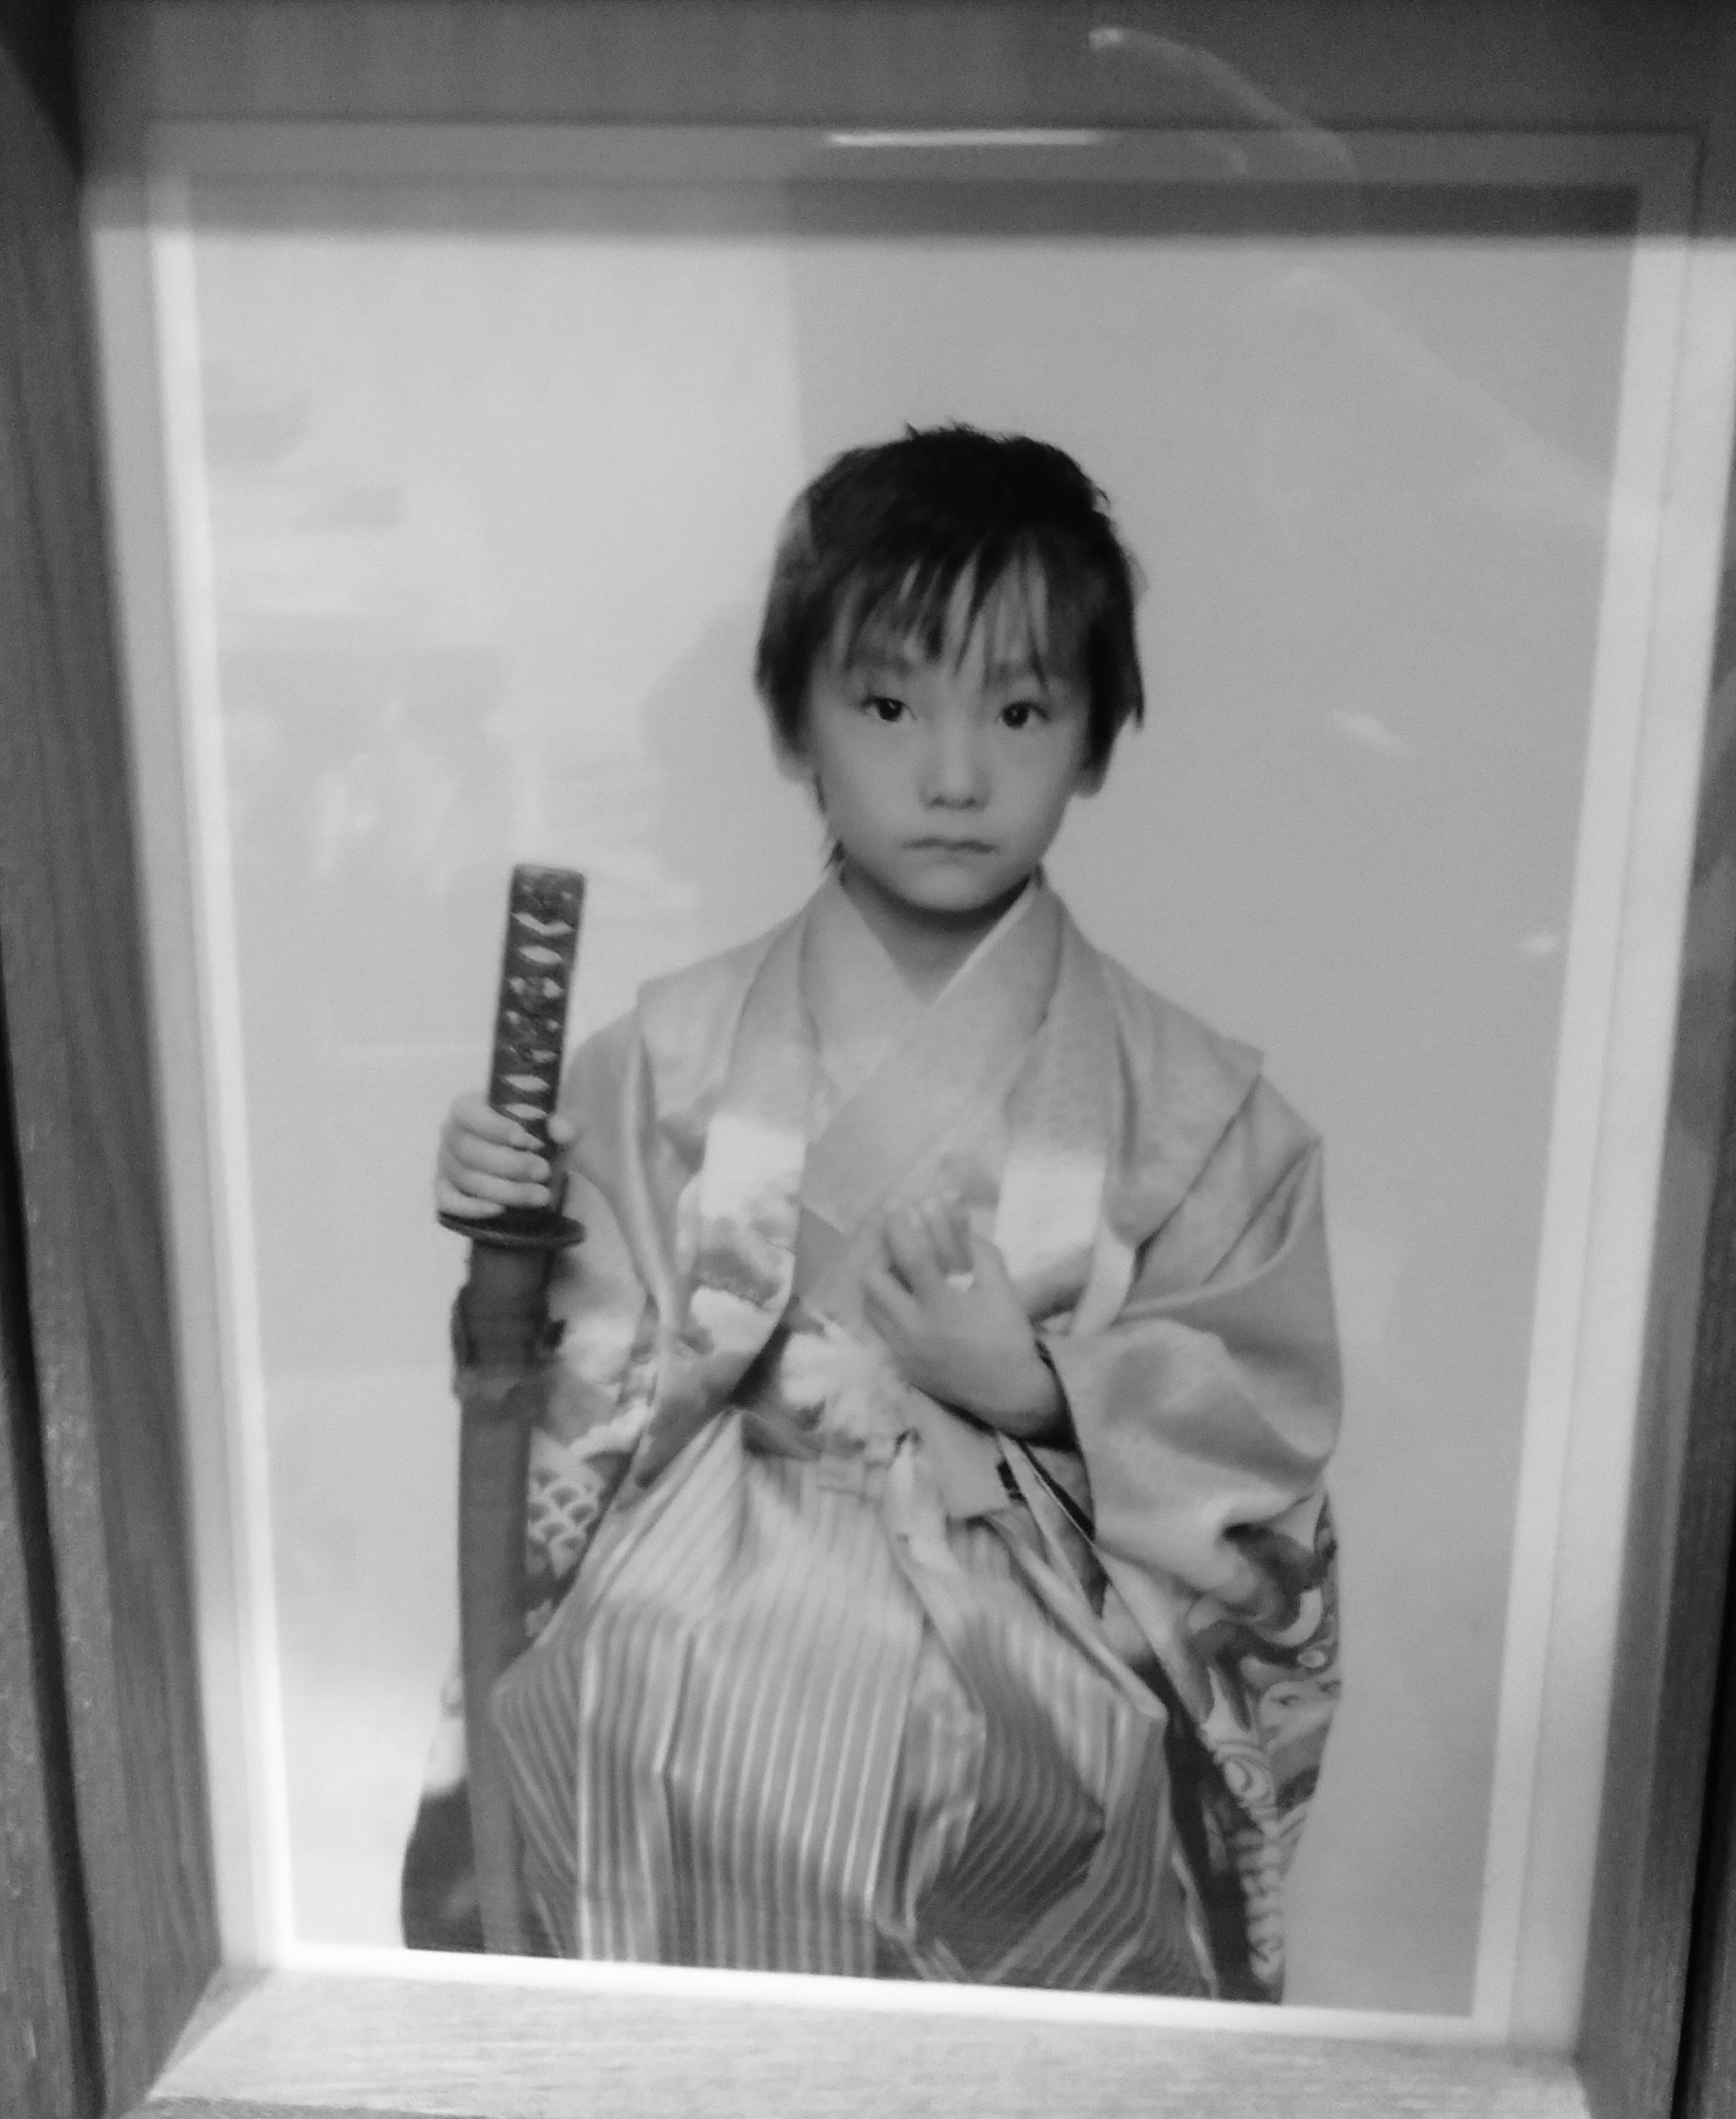
\includegraphics[scale=0.065]{figures/before.jpeg}
                \end{center}
            \end{column}
            \begin{column}{.5\linewidth}
                \centering{after}
                \begin{center}
                    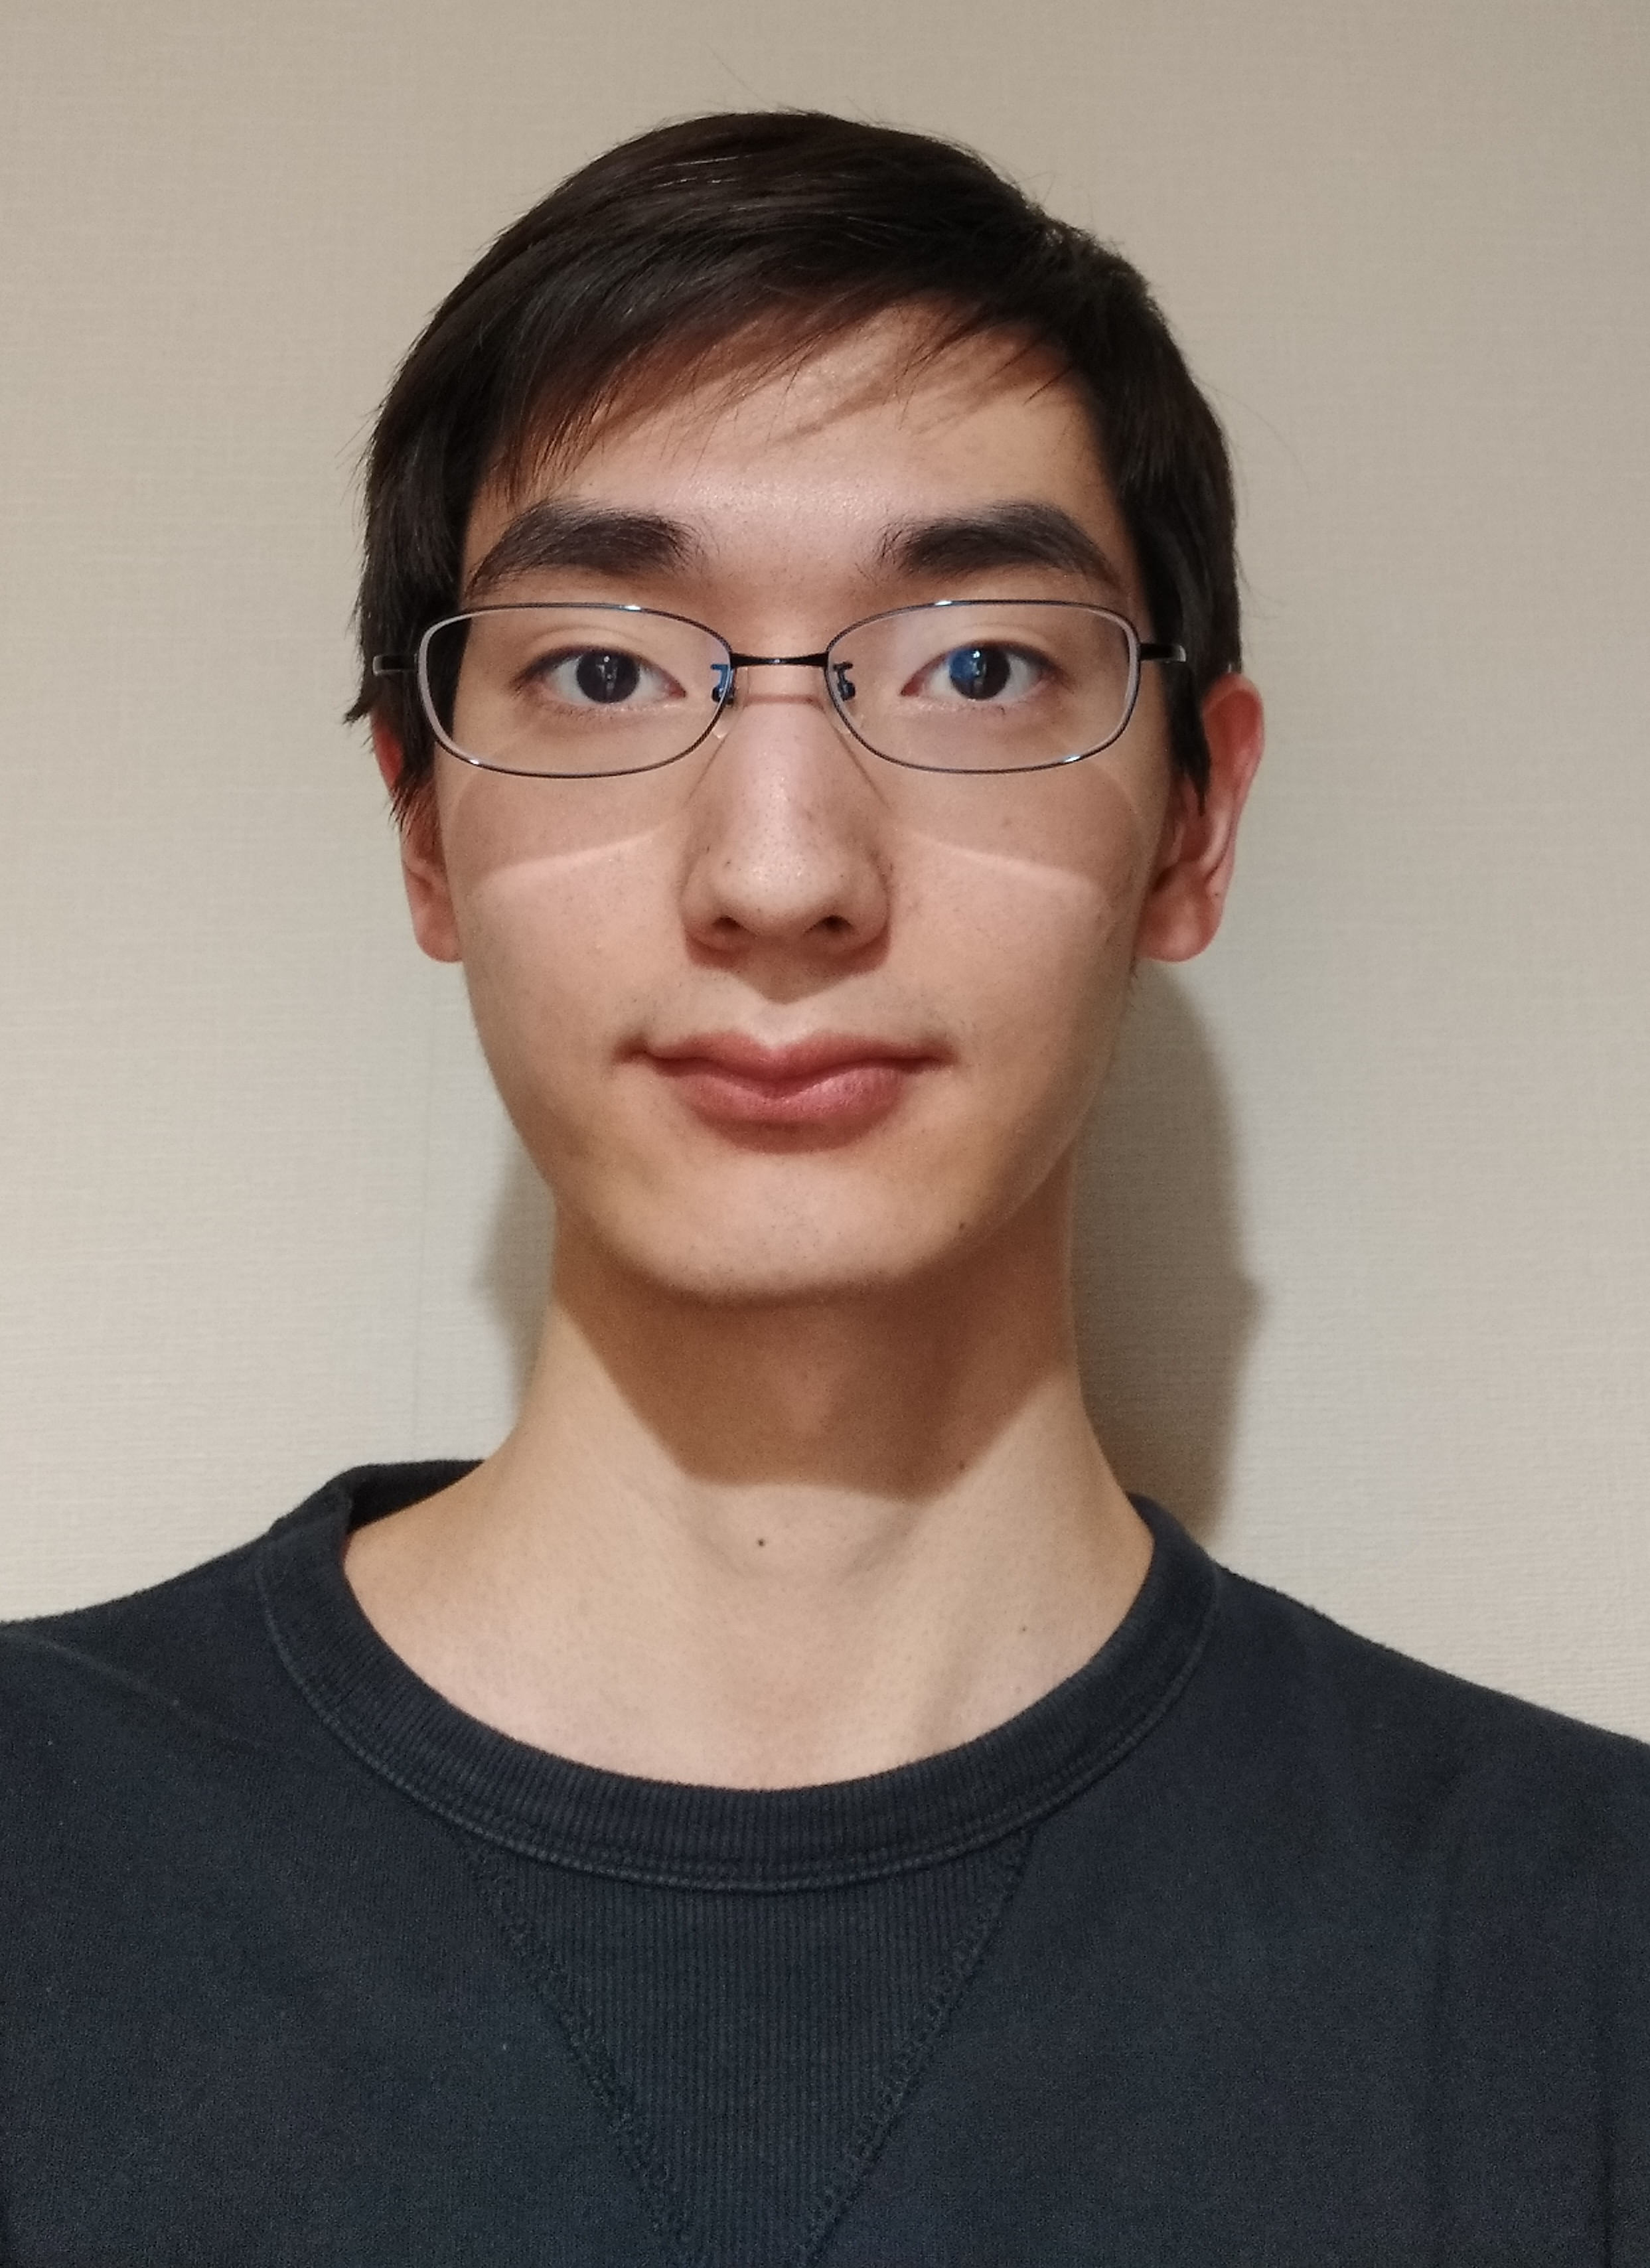
\includegraphics[scale=0.045]{figures/after.jpeg}
                \end{center}
            \end{column}
        \end{columns}
    \end{frame}

    % 自己紹介スライド
    \begin{frame}{経歴とか}
        \begin{columns}
            \begin{column}{.5\linewidth}
                \begin{itemize}
                    \item 名前: 竹本 志恩
                    \item 出身: 東京都
                    \item 居住: 中央区
                    \item 高校
                    \begin{itemize}
                        \item 芝浦工業大学附属
                        \item 今度大学でTOEIC受験します
                        \item 気まずい...
                    \end{itemize}
                \end{itemize}          
            \end{column}
            \begin{column}{.4\linewidth}
                \begin{center}
                    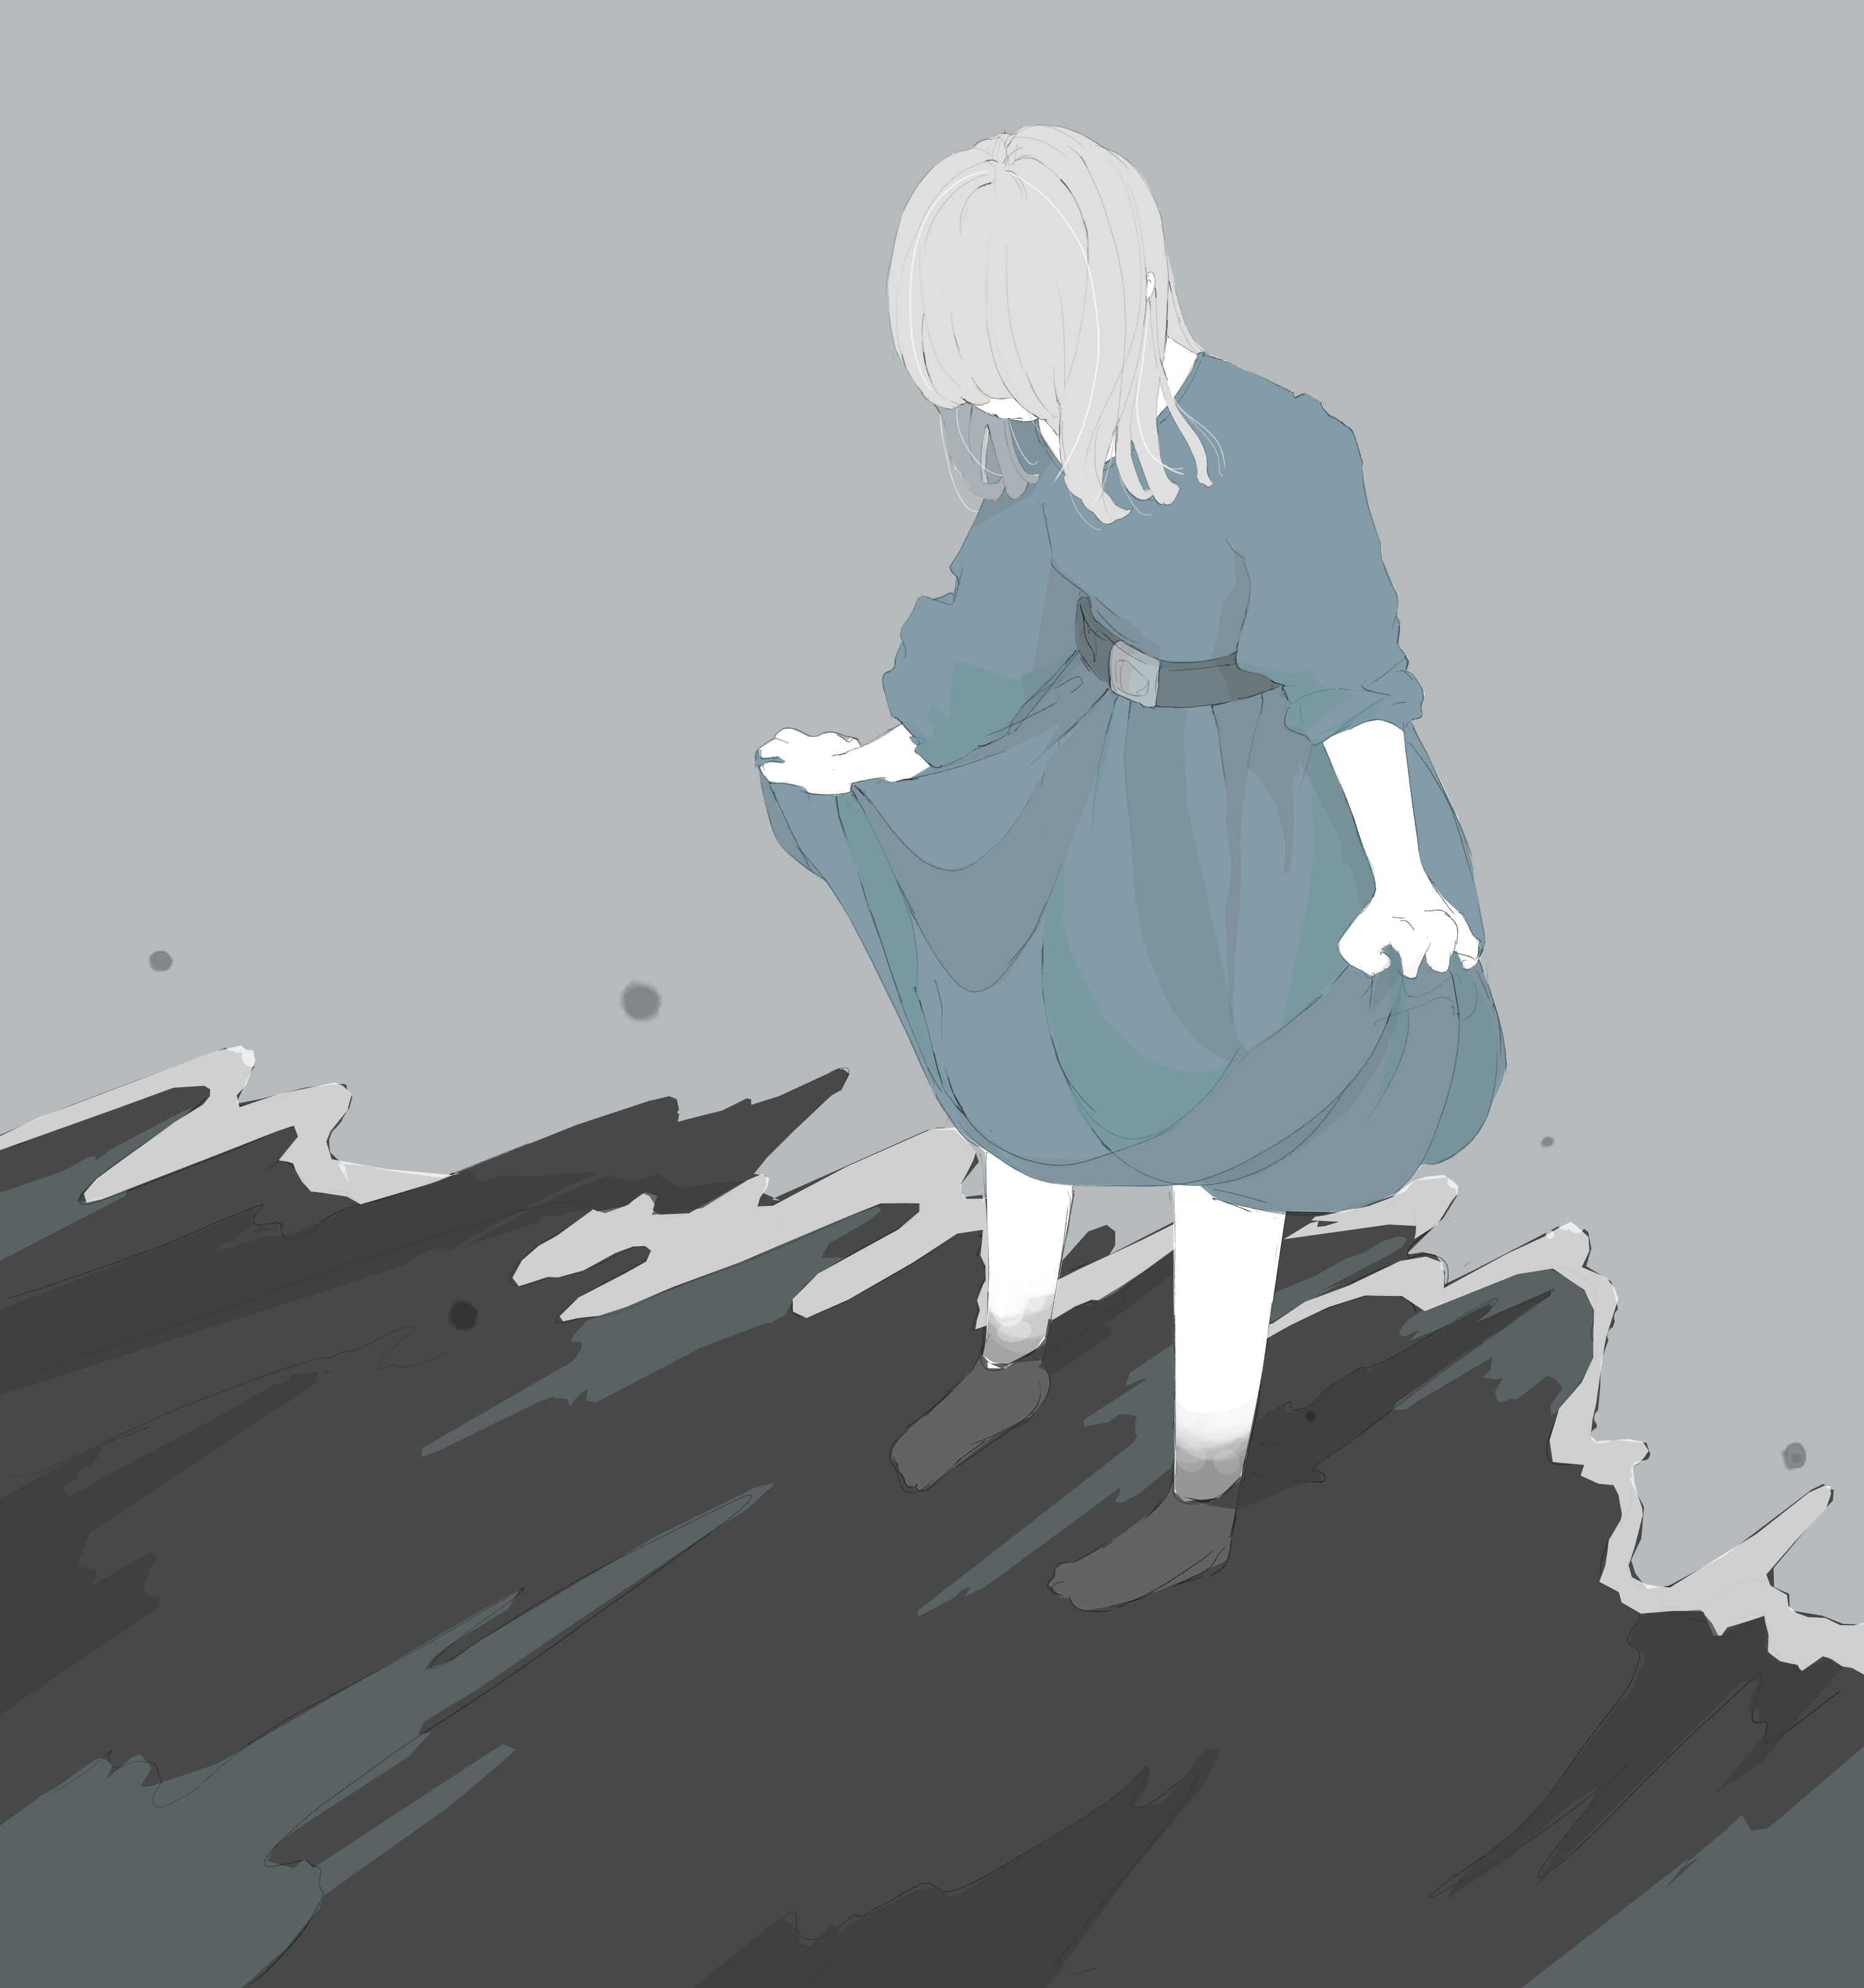
\includegraphics[height=40mm, width=40mm]{figures/444.jpeg}
                \end{center}
                \centering{\scriptsize {闇打ち際}}
                \centering{\scriptsize {https://fromtheasia.com/illustration/nocopyrightgirl}}
            \end{column}
        \end{columns}
    \end{frame}


    %好きなこと
    \begin{frame}{好きなこともの-1}
        \begin{columns}
            \begin{column}[]{.5\linewidth}
                \begin{itemize}
                    \item 考える
                    \item 歩く
                    \item 食べる
                    \begin{itemize}
                        \item 近頃は蕎麦
                        \item ここ数年,生姜が好き
                    \end{itemize}
                    \item 書く
                    \begin{itemize}
                        \item 考えとか色々
                        \item 知的生産に興味あり
                    \end{itemize}
                \end{itemize}
            \end{column}
            \begin{column}[]{.5\linewidth}
                \begin{center}
                    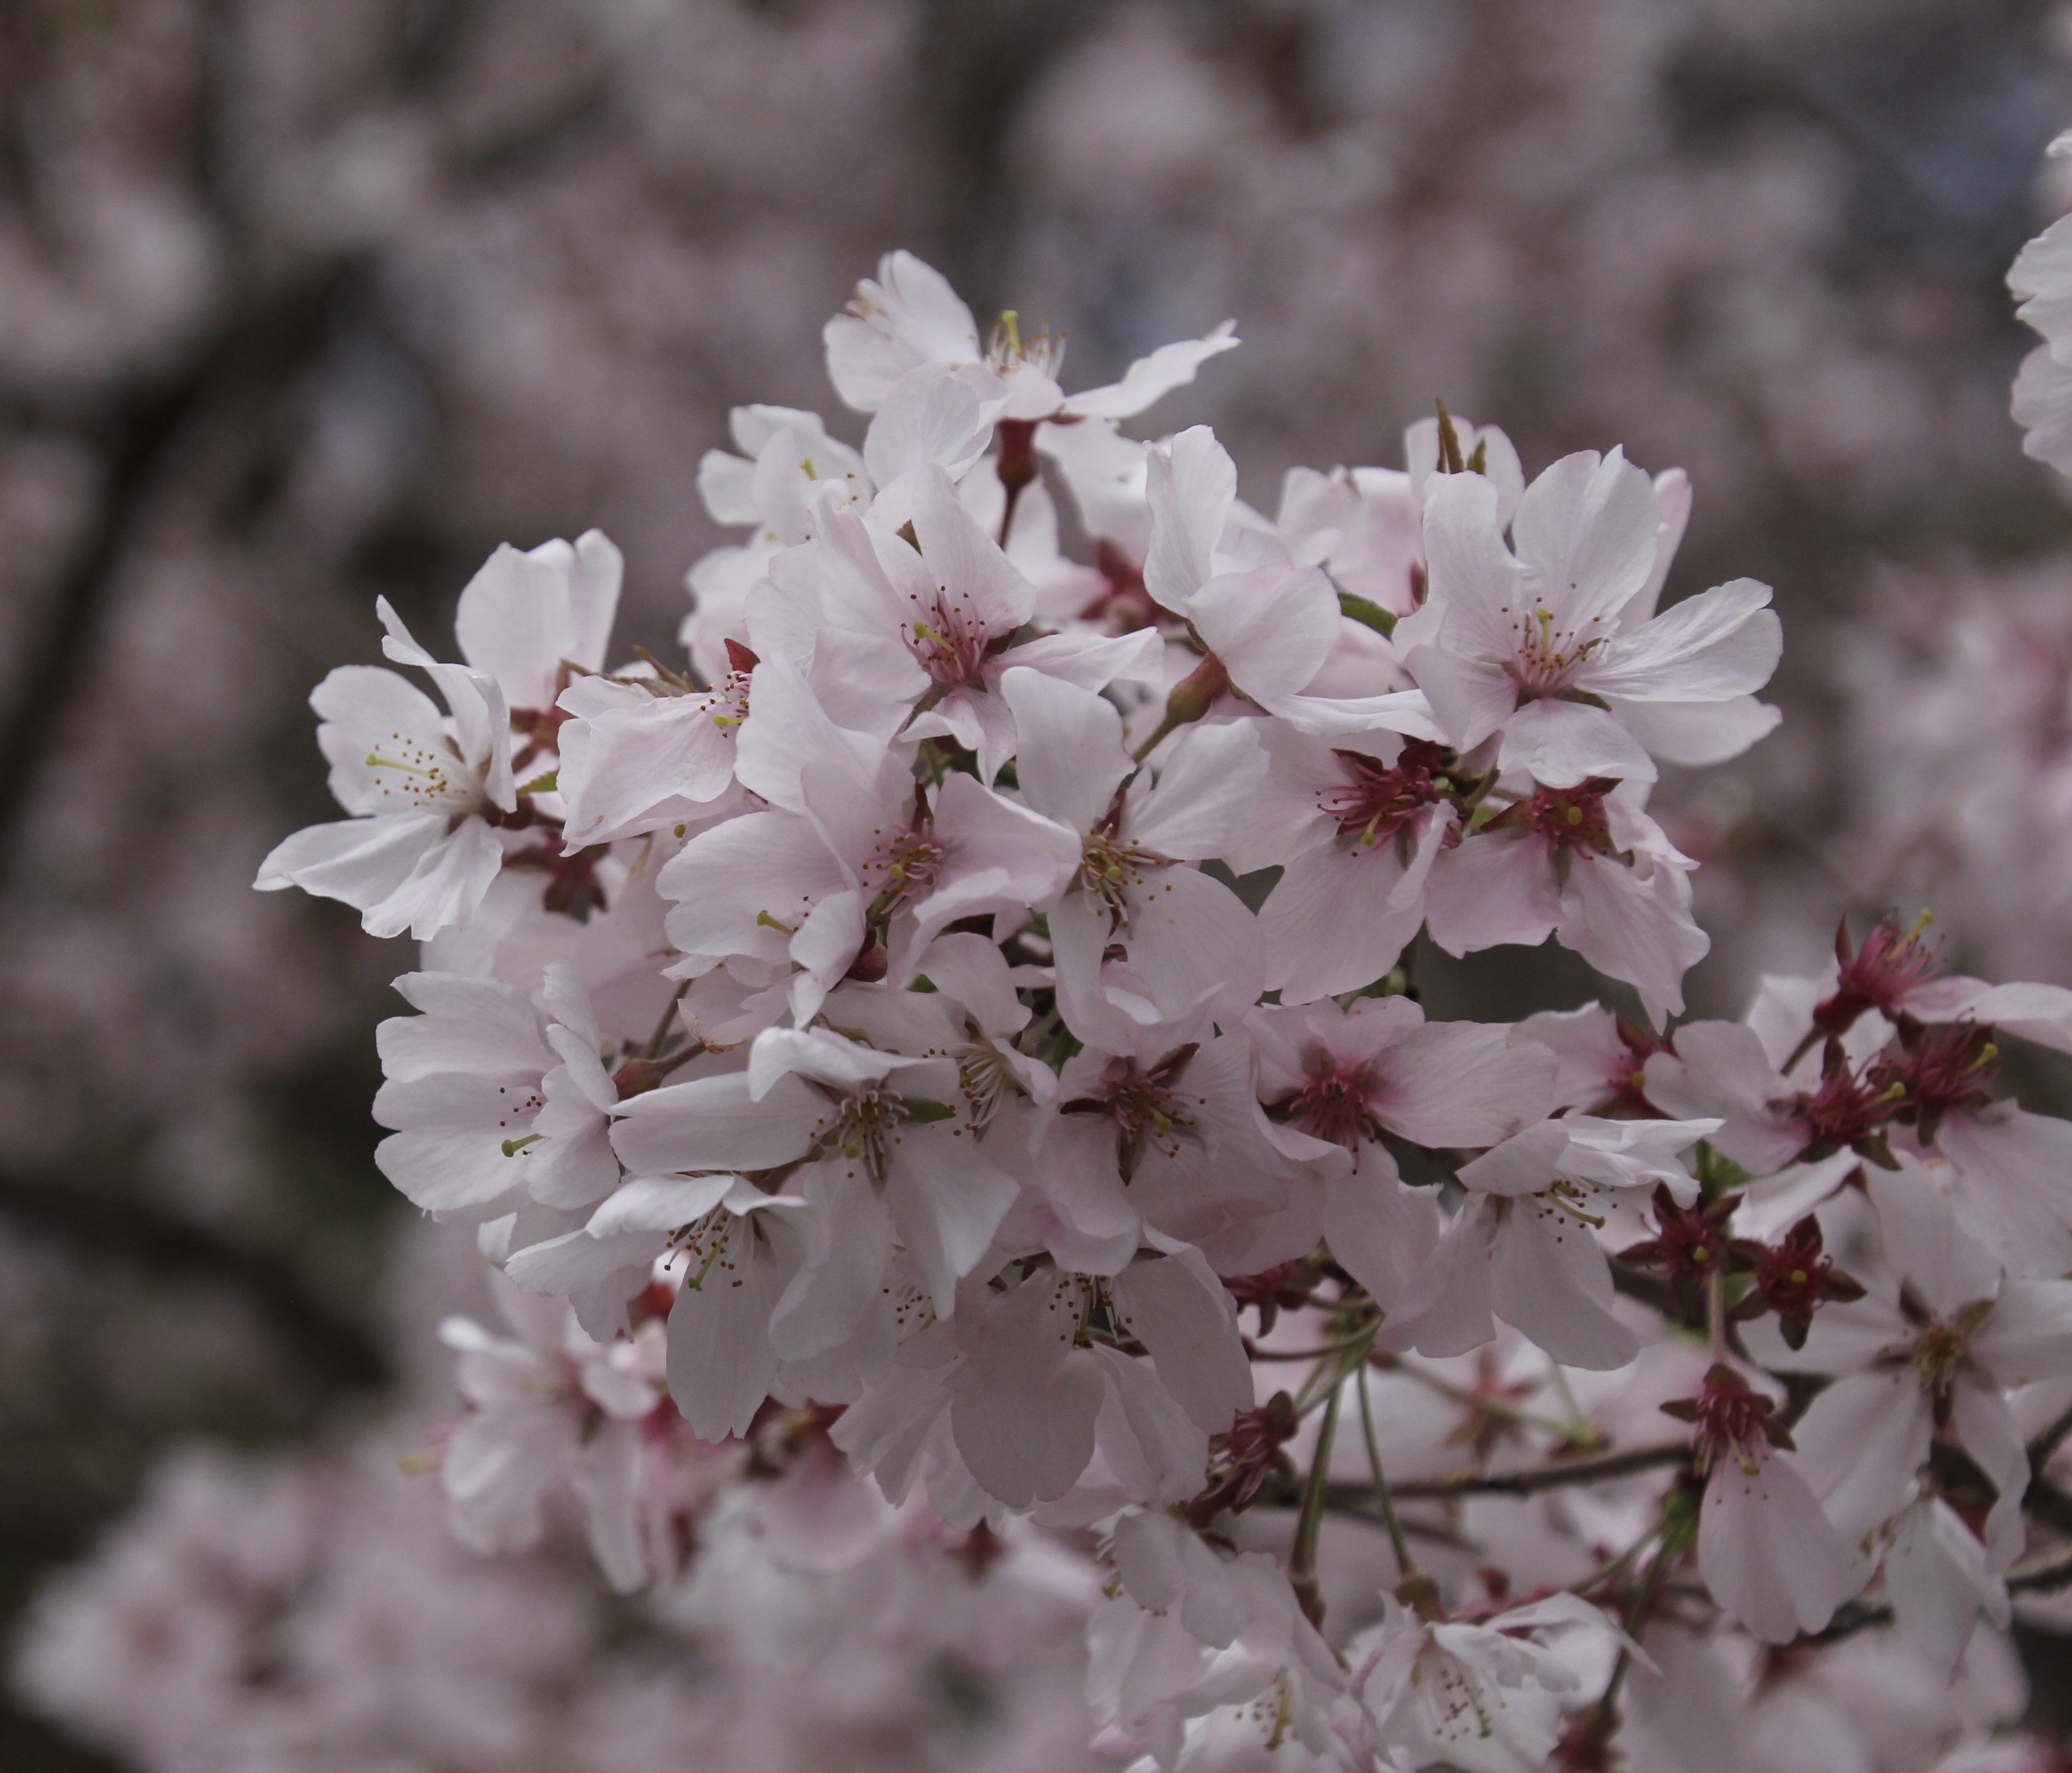
\includegraphics[scale=0.05]{figures/sakura1.jpeg}
                    \scriptsize{蕎麦の代わり}
                \end{center}
            \end{column}
        \end{columns}
    \end{frame}

    \begin{frame}{好きなこともの-2}
        \begin{columns}
            \begin{column}[]{.5\linewidth}
                \begin{itemize}
                    \item 読む
                    \begin{itemize}
                        \item 小説
                        \item 随筆
                        \item 何かの記事
                        \item ブログ
                    \end{itemize}
                    \item 色々やる
                    \begin{itemize}
                        \item 体験を得て考える
                        \item vimとRustがあまり進んでない
                        \item ここ数日はlatex
                        \item スライドもlatex製
                    \end{itemize}
                \end{itemize}
            \end{column}
            \begin{column}[]{.5\linewidth}
                \begin{center}
                    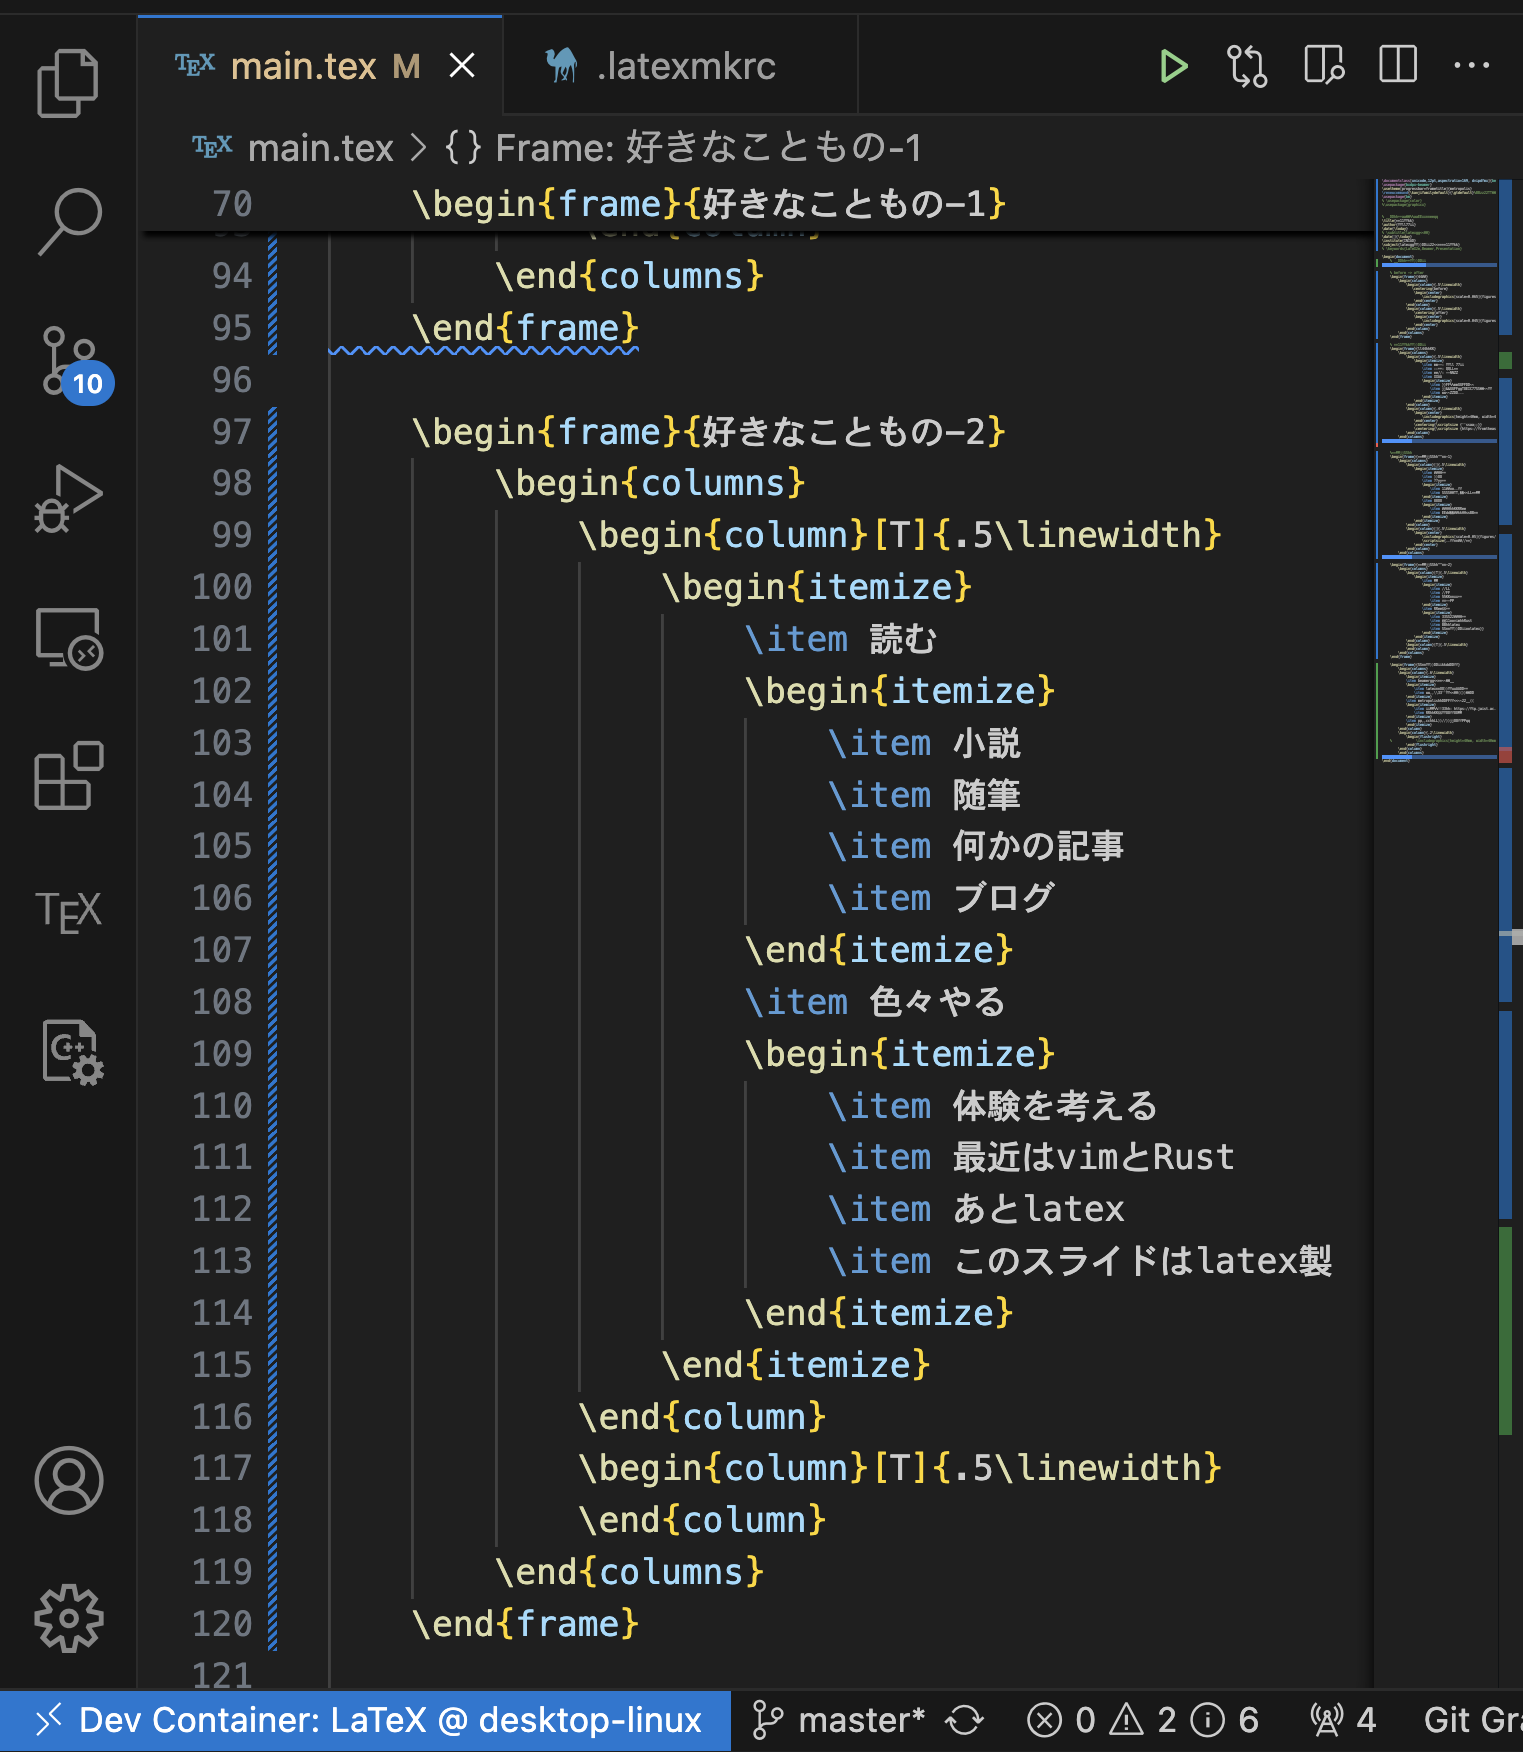
\includegraphics[scale=0.25]{figures/latex.png}
                \end{center}
            \end{column}
        \end{columns}
    \end{frame}

    \begin{frame}{このスライドについて}
        \begin{columns}
        \begin{column}{\linewidth}
            \begin{itemize}
            \item beamerで作りました
            \begin{itemize}
                \item latexのクラスファイル
                \item プレゼン資料作成用らしい
            \end{itemize}
            \item metropolisというテーマを使用
            \begin{itemize}
                \item ドキュメント: https://ftp.jaist.ac.jp/pub/CTAN/macros/latex/contrib/beamer-contrib/themes/metropolis/doc/metropolistheme.pdf
                \item 割と見やすくて良い
            \end{itemize}
            \item バレットが変わらなくて困惑
            \item パワポとどちらが良いか考えたい
            \end{itemize}          
        \end{column}
        \end{columns}
    \end{frame}
\end{document}